\documentclass[a4paper,10pt]{report}
\usepackage[utf8]{inputenc}
\usepackage{graphicx}
\usepackage[francais]{babel}
\usepackage{color}

% Title Page
\title{Annexes}
\author{Adrien DROGUET}


\begin{document}
\maketitle

\tableofcontents
\pagebreak

\chapter{Diagrammes de classe}

\section{core}
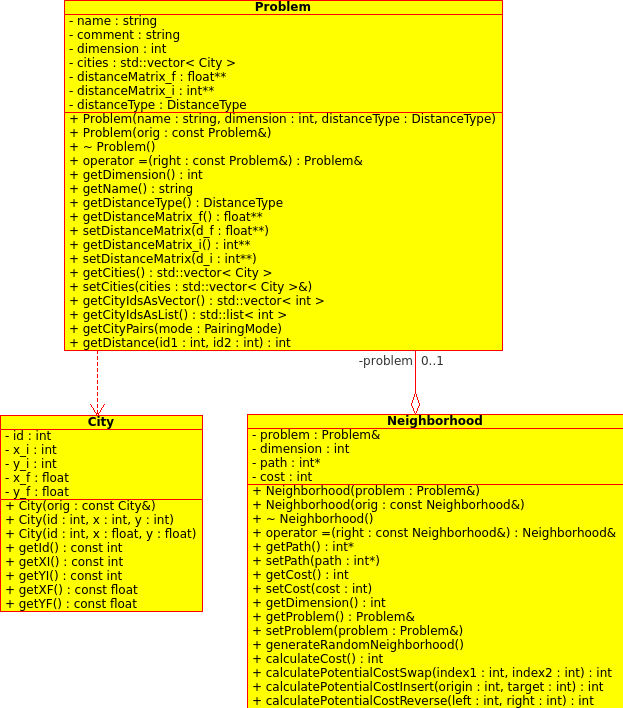
\includegraphics[width=\textwidth]{../UML/core.png}

\paragraph{}
\textbf{Problem} contient une matrice de distance, calculée une fois que toutes
les citées ont été enregistrées, qui va être l'attribut le plus important de
\textbf{Problem}, réutilisé par toutes les méthodes de calcul de coût.

\section{relation}
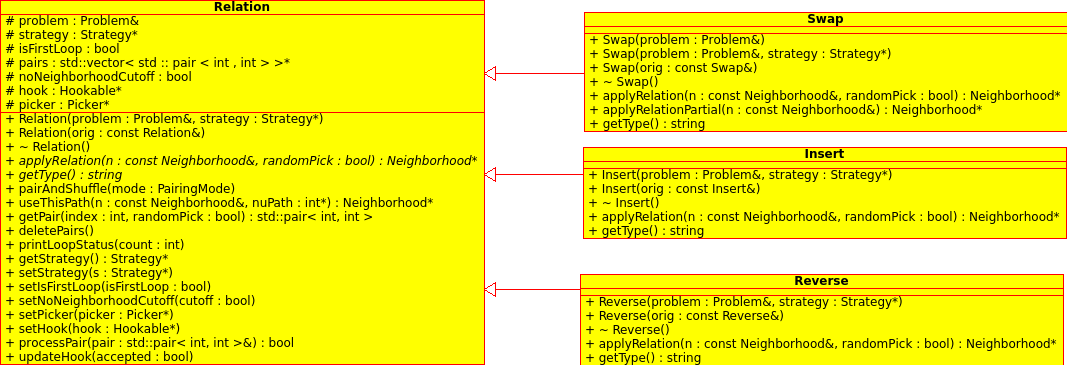
\includegraphics[width=\textwidth]{../UML/relation.png}

\section{strategy}
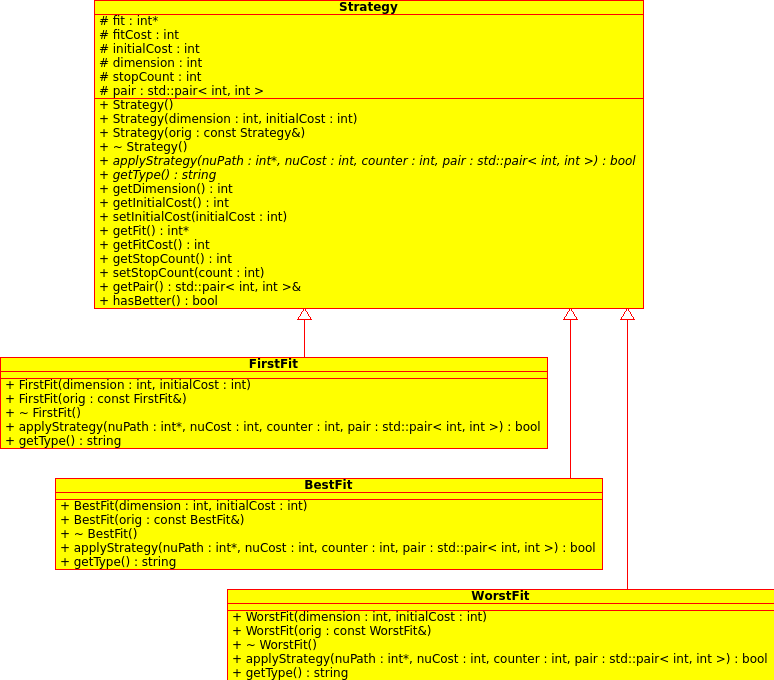
\includegraphics[width=\textwidth]{../UML/strategy.png}

\section{run}
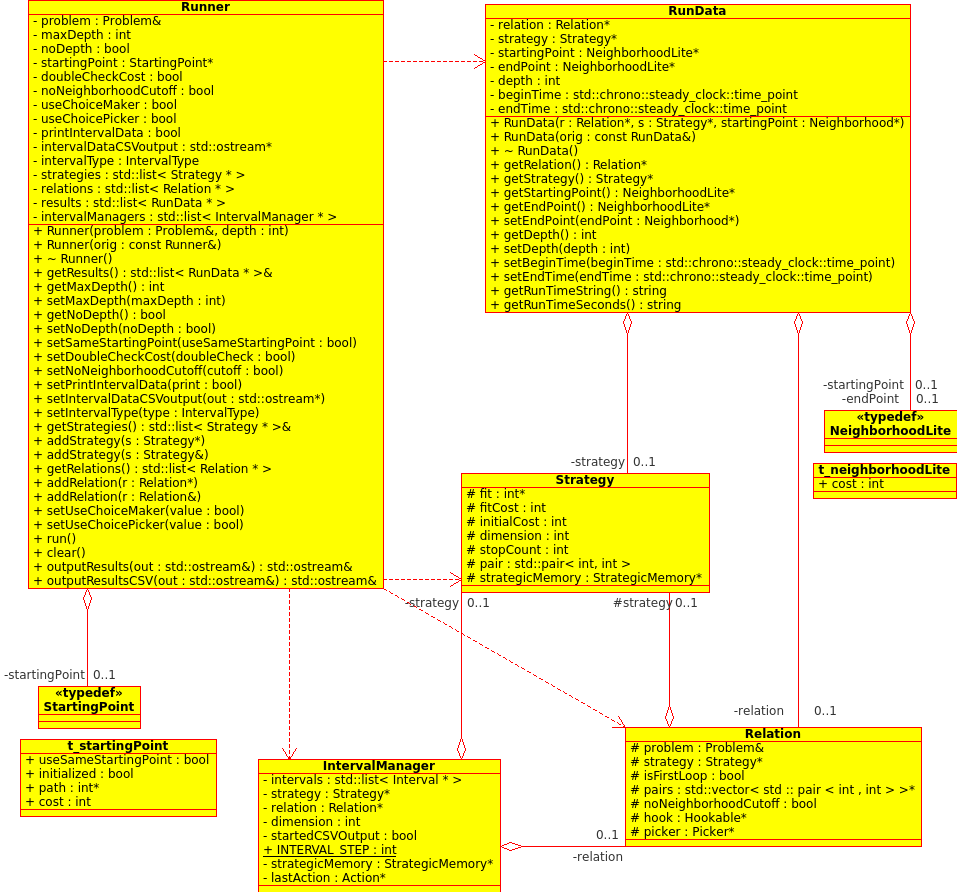
\includegraphics[width=\textwidth]{../UML/run.png}

\subsection{interval}
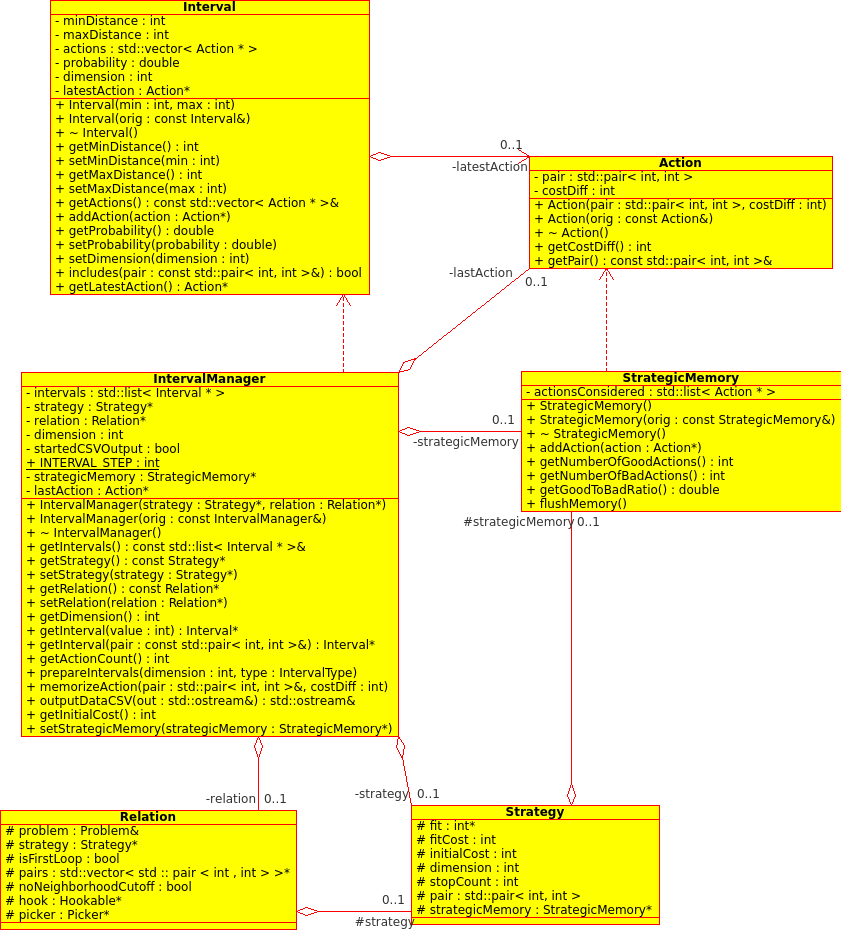
\includegraphics[width=\textwidth]{../UML/interval.png}

\section{hook}
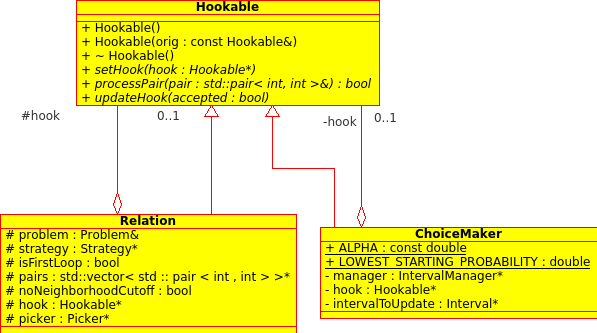
\includegraphics[width=\textwidth]{../UML/hook.png}

\section{choice}
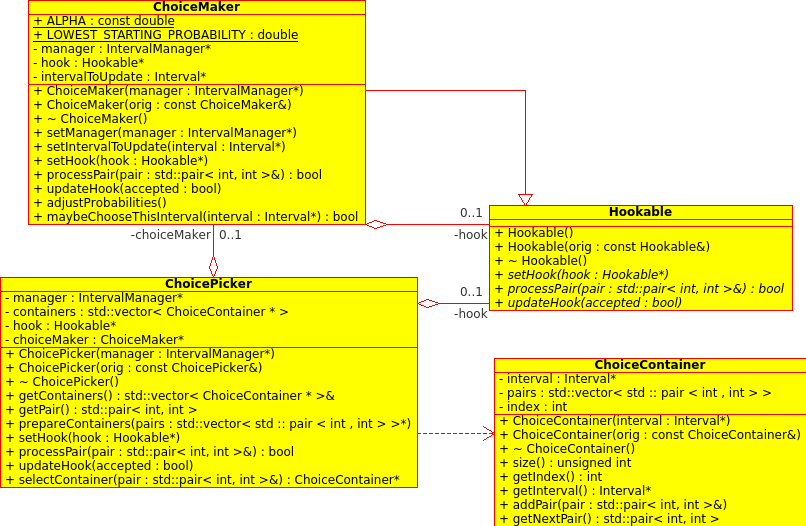
\includegraphics[width=\textwidth]{../UML/choice.png}



\chapter{Données et Résultats d'exécution}

\section{Représentation des TSP}

\begin{figure}[h]

NAME: burma14\\
TYPE: TSP\\
COMMENT: 14-Staedte in Burma (Zaw Win)\\
DIMENSION: 14\\
EDGE\_WEIGHT\_TYPE: GEO\\
EDGE\_WEIGHT\_FORMAT: FUNCTION \\
DISPLAY\_DATA\_TYPE: COORD\_DISPLAY\\
NODE\_COORD\_SECTION\\
\begin{tabular}{rlcr}
 1&  16.47&&       96.10\\
 2&  16.47&&       94.44\\
 3&  20.09&&       92.54\\
 4&  22.39&&       93.37\\
 5&  25.23&&       97.24\\
 6&  22.00&&       96.05\\
 7&  20.47&&       97.02\\
 8&  17.20&&       96.29\\
 9&  16.30&&       97.38\\
10&  14.05&&       98.12\\
11&  16.53&&       97.38\\
12&  21.52&&       95.59\\
13&  19.41&&       97.13\\
14&  20.09&&       94.55\\
\end{tabular}
\\EOF
\caption{burma14.tsp}
\end{figure}


\section{Résultats moyens}

\paragraph{}
  Les tableaux ci-dessous représente la compilation des résultats d'une
quarantaine d'exécutions.

\begin{figure}[h]
  \begin{center}
    \begin{tabular}{|l|r|r|r|}
      \hline
      &		\textbf{First Fit}&	\textbf{Best Fit}&	\textbf{Worst
Fit}\\\hline
      \textbf{Swap}&
	  6 012,195&
	  6 610,488&
	  \textbf{\textcolor{blue}{6 007,561}}\\\hline
      \textbf{Insert}&
	  \textbf{\textcolor{blue}{4 560,732}}&
	  4 804,634&
	  4 663,171\\\hline
      \textbf{Reverse}&
	  4 389,024&
	  \textbf{\textcolor{blue}{4 388,293}}&
	  4 416,341\\\hline
    \end{tabular}
    \caption{Résultats moyens pour le TSP berlin52}
  \end{center}
\end{figure}

\begin{figure}[H]
  \begin{center}
    \begin{tabular}{|l|r|r|r|}
      \hline
      &		\textbf{First Fit}&	\textbf{Best Fit}&	\textbf{Worst
Fit}\\\hline
      \textbf{Swap}&
	  204 979,051&
	  216 486,103&
	  \textbf{\textcolor{blue}{198 029,436}}\\\hline
      \textbf{Insert}&
	  \textbf{\textcolor{blue}{168 662,564}}&
	  174 234,641&
	  \textbf{169 584,231}\\\hline
      \textbf{Reverse}&
	  154 457,282&
	  \textbf{\textcolor{blue}{151 268,590}}&
	  158 711,872\\\hline
    \end{tabular}
    \caption{Résultats moyens pour le TSP bier127}
  \end{center}
\end{figure}

\begin{figure}[h]
  \begin{center}
    \begin{tabular}{|l|r|r|r|}
      \hline
      &		\textbf{First Fit}&	\textbf{Best Fit}&	\textbf{Worst
Fit}\\\hline
      \textbf{Swap}&
	  6 367,200&
	  6 989,250&
	  \textbf{\textcolor{blue}{5 497,750}}\\\hline
      \textbf{Insert}&
	  3 647,000&
	  4 368,950&
	  \textbf{\textcolor{blue}{3 484,050}}\\\hline
      \textbf{Reverse}&
	  \textbf{\textcolor{blue}{2 855,500}}&
	  \textbf{2 856,250}&
	  2 859,800\\\hline
    \end{tabular}
    \caption{Résultats moyens pour le TSP ch130}
  \end{center}
\end{figure}

\begin{figure}[H]
  \begin{center}
    \begin{tabular}{|l|r|r|r|}
      \hline
      &		\textbf{First Fit}&	\textbf{Best Fit}&	\textbf{Worst
Fit}\\\hline
      \textbf{Swap}&
	  7 774,650&
	  7 876,250&
	  \textbf{\textcolor{blue}{5 949,600}}\\\hline
      \textbf{Insert}&
	  4 253,050&
	  5 281,000&
	  \textbf{\textcolor{blue}{3 752,950}}\\\hline
      \textbf{Reverse}&
	  3 257,550&
	  \textbf{\textcolor{blue}{3 257,200}}&
	  3 264,750\\\hline
    \end{tabular}
    \caption{Résultats moyens pour le TSP ch150}
  \end{center}
\end{figure}

\section{Graphes d'exécution}

\begin{figure}[h]
  \begin{center}
    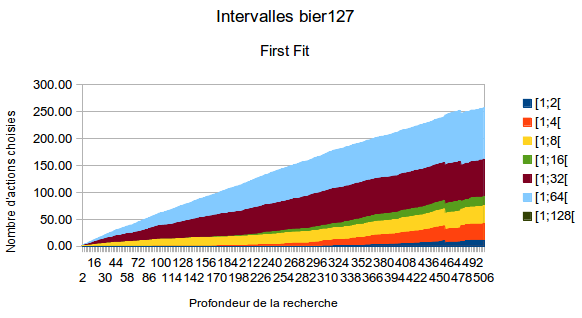
\includegraphics[width=\textwidth]{images/bier127-intervals-first-fit.png}
  \end{center}
\end{figure}

\begin{figure}[h]
  \begin{center}
    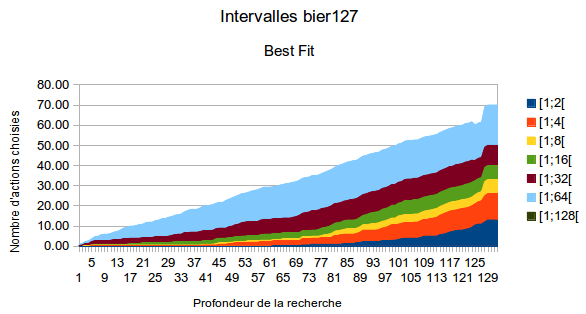
\includegraphics[width=\textwidth]{images/bier127-intervals-best-fit.png}
  \end{center}
\end{figure}

\begin{figure}[h]
  \begin{center}
    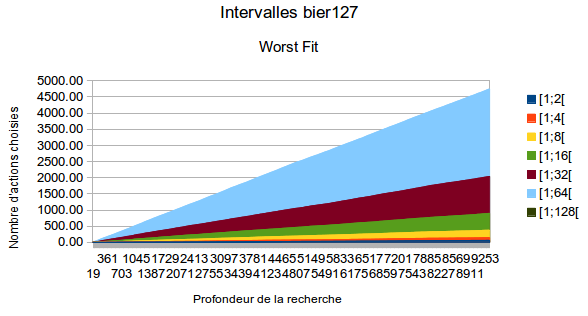
\includegraphics[width=\textwidth]{images/bier127-intervals-worst-fit.png}
  \end{center}
\end{figure}

\subsection{Portée}

%+extra cost & intervals

\chapter{Divers}
\section{Arguments de lancement (liste non exhaustive)}

\begin{itemize}
 \item \textbf{-file [nom de fichier]} ==\textgreater TSP à optimiser
 \item \textbf{-maxDepth [entier]} ==\textgreater spécifie une profondeur de
recherche maximale
 \item \textbf{-noMaxDepth} ==\textgreater 
 \item \textbf{-r [swap|insert|reverse]} ==\textgreater  ajoute un voisinage à
explorer
 \item \textbf{-s [firstFit|bestFit|worstFit]} ==\textgreater ajoute une
stratégie à appliquer
 \item \textbf{-o [nom de fichier|auto]} ==\textgreater spécifie un fichier de
sortie ou laisse le programme décider d'un nom de fichier (recommandé)
 \item \textbf{-saveIntervalData} ==\textgreater enregistre les données
d'intervalle lors de l'exécution ; si un fichier de sortie a été spécifié, la
trace d'exécution sera sauvée en tant que \textless nom\textgreater.csv.i
 \item \textbf{-intervalStep [entier]} ==\textgreater spécifie une puissance de
croissance de la taille des intervalles (4 par défaut)
 \item \textbf{-intervalType [disjoint|joined\_at\_origin]} ==\textgreater
spécifie le type d'intervalle à enregistrer (joined\_at\_origin recommandé)
 \item \textbf{-sameStartingPoint} ==\textgreater utiliser le même point de
départ pour chaque algorithme
 \item \textbf{-doubleCheckCost} ==\textgreater force un calcul complet des
coûts en fin d'exécution ; envoie un message d'erreur si il y a des
irrégularités
\end{itemize}


\end{document}          
